\documentclass[a4paper, english, fullpage]{article}


% FOR UTF-8?
\usepackage{ucs}
\usepackage{here}   %Put figs at location when using H
\usepackage[utf8x]{inputenc}
\usepackage[english]{babel}
\usepackage{amsmath}
\usepackage{verbatim}
\usepackage{graphicx}
\usepackage[final]{pdfpages}
\graphicspath{{./images/}}

%Paragraph settings
\setlength{\parindent}{0pt}
\setlength{\parskip}{12pt plus2pt minus2pt}

%Nicer margins
\addtolength{\voffset}{-35pt}
\addtolength{\textheight}{75pt}

% No windows or orphans
\widowpenalty=500
\clubpenalty=500

%Commands
\newcommand{\unit}[1]{\ensuremath{\, \mathrm{#1}}}

\begin{document}
%%%%%%%%%%%%%%%%%%%%%%%%%%%%%%%%%%%%%%%%%%%%%%%%%%%%%%%%%%%%%%%%%%%%%%%
% FRAMSIDA
\title{{\Huge Avoiding phantom jams in traffic}\\[0.5cm]
- Simulations with agent-based models}
\date{December 18, 2009}
\author{Simon Lindkvist \and Sebastian Johansson}
 
\maketitle
%%%%%%%%%%%%%%%%%%%%%%%%%%%%%%%%%%%%%%%%%%%%%%%%%%%%%%%%%%%%%%%%%%%%%%%
%% SAMMANFATTNING
%\newpage
\begin{abstract}
Det här är en sammanfattning. Test of reference to \cite{sugiyama}.
\end{abstract}




%Introduction and problem definition
%	Phantom jams
\section{Introduction}

Huge amounts of resources are used every year to build and maintain roads
around the globe. The Swedish Road Administration alone, has a annual budget
of 21 billion SEK \cite{vagverket}. Reducing traffic jams, and thereby
reducing the need for building new roads is highly motivated.\\\\

\begin{figure}[H]
    \begin{center}
    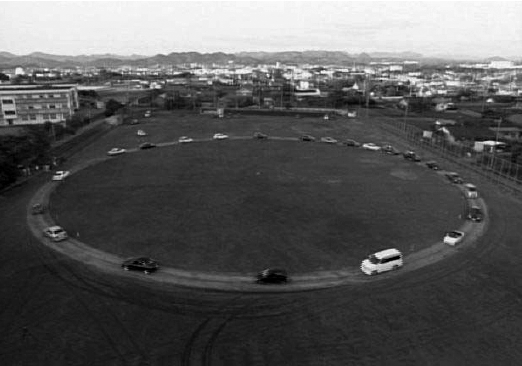
\includegraphics[width=0.75\textwidth]{sug_circlephoto.png}
    \caption{\label{sug_photo}
Experiment by Y. Sugiyama el al. \cite{sugiyama}. 22 cars on a circular road
of length 230 m. A traveling phantom jam has appeared and can now bee seen in
the upper-right part of the photo.
} \end{center} \end{figure}

In free flowing traffic, traffic jams can appear for no apparent reason. Even
without the presence of bottle-necks such as traffic-lights, crossroads or
slip roads. In light traffic, drivers adjust to any
instabilities, but as soon as traffic reaches a certain level of density, jams
occur. This phenomena is known as jamitons or \emph{phantom jams} and has
recently been confirmed experimentally by Y. Sugiyama et al. (see fig
\ref{sug_photo} and \ref{sug_positions}) \cite{sugiyama}. Once a phantom jam has been
established, the jam travels backwards in traffic as a wave. Recently it was
shown by M. R. Flynn et al. \cite{mit} that these waves are mathematically
similar to travelling shock-waves caused by explosions.\\\\

\begin{figure}[H]
    \begin{center}
    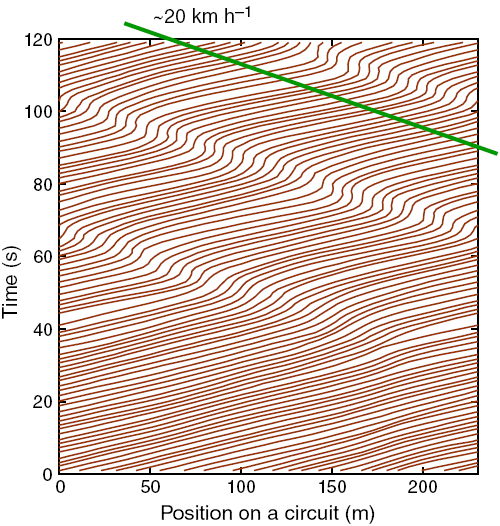
\includegraphics[width=0.6\textwidth]{sug_positions.png}
    \caption{\label{sug_positions}
Data measured during the experiment seen in fig \ref{sug_photo}. A disturbance
can be seen after 40 s and is quickly amplified into a phantom jam, travelling
backwards around the circle at approximately 20 km/h.
Diagram by Y. Sugiyama el al. \cite{sugiyama}.}
\end{center} \end{figure}

Traffic flow and thereby the efficiency of roads, is severely reduced by
traffic jams such as phantom jams (see fig \ref{sug_flow}) \cite{sugiyama}. If we implement a system that shifts the critical level of traffic density at which phantom jams occur upwards, we improve road efficiency. In this report we evaluate two such systems: Adaptive Cruise Control and an improved version that we have named Enhanced Adaptive Cruise Control. Results are taken from our simulator based on agent-based modelling.

\begin{figure}[H]
    \begin{center}
    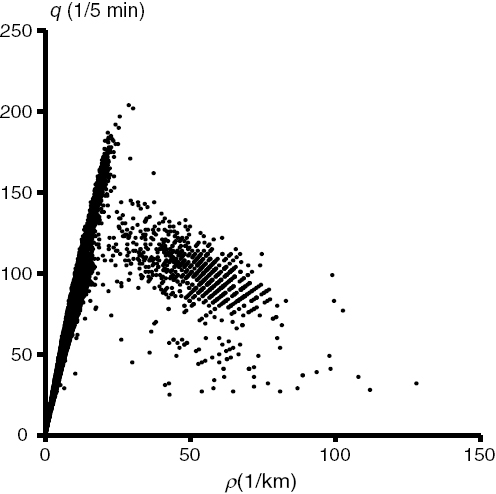
\includegraphics[width=0.6\textwidth]{sug_trafficFlow.png}
    \caption{\label{sug_flow}
Traffic flow as a function of traffic density. The data is clearly divided
into two sets, one representing free flowing traffic and the other (above the
threshold of 25 vehicles per km) representing congested traffic (with traffic
jams).  Results from article by Y. Sugiyama el al. \cite{sugiyama}.  Data was
measured by Japan Highway Public Cooperation on Japanese highways. Similar
observations have been made in many places and seems to be almost a universal
property of highway traffic.}
    \end{center}
\end{figure}

	

%Driver model
\section{Driver model}
Several driver models have been developed to simulate different traffic situations. These models describe the position and velocity of each car in the simulation and can then much easier be compared with empirical data than in macroscopic models. Intelligent Driver Model (IDM) is a car-following model and belongs to the deterministic kind of microscopic models.

The IDM control the position of the car on a single-lane road. The position depends on the velocity and acceleration of the car. Acceleration is described by the velocity \begin{math}v_\alpha\end{math} and distance to the car in front \begin{math}s_\alpha\end{math}. These two parts are related to the desired velocity \begin{math}v_0\end{math} and effective desired distance \begin{math}s^\ast\end{math}. The equation for acceleration then becomes:
\begin{math}\dot{v_\alpha} = a(1-(\frac{v_\alpha}{v_0})^\delta-(\frac{s^\ast}{s_0})^2)\end{math}
Desired distance between the cars is calculated from minimum distance \begin{math}s_0\end{math}, time headway \begin{math}T\end{math} and difference in velocity \begin{math}\Delta v\end{math}.
\begin{math}s^\ast = s_0 + max(v_\alpha T + \frac{v_\alpha \Delta v}{2\sqrt{ab}})\end{math}

%Methods to reduce
\section{Methods to reduce jams}
A technology to increase safety for drivers in traffic is Adaptive Cruise Control (ACC) which is the next generation of cruise control. This kind of system is able to measure the distance and speed to the car infront and then adapt the speed so a certain time gap is maintained between the cars. ACC is already commercially available on the market and there is much research going on to see the effect in traffic flow when more and more vehicles are equipped with this system \cite{acc}.

%Simulator and implementation of the three methods
\section{Simulator setup}
In the created simulator we had a one-lane circular road with a length of
800 m. Different amounts of cars could be placed on the track corresponding to
a certain traffic density. During one simulation this meant that the density
was constant since no cars could be added or removed during one run. Initially
all cars were positioned equally spaced on the circular road, but then every car
was moved forward randomly between 0 and 1 metre to create some initial
perturbation. This speeded up the emergence of phantom jams. The graphical user
interface of the simulator can be seen in Appendix \ref{gui}.

\subsection{Implementation of mathematical models}
The Intelligent Driver Model has been used as basis for the control system
for all agents (cars). We have done simulations with three different versions.

\begin{comment}
The three systems described in Sections (FIXME: ref till dessa tre modeller)
were implemented as described below. Since the simulator used a circular road
position of the car was transformed into an angle from 0 to 2\begin{math}\pi
\end{math} but since the acceleration and velocity were not affected by this,
the car was only aware of a straight road where the car going out in one
end started over from the other end.
\end{comment}

\subsubsection {Normal driver}
The IDM was developed to describe a normal behavior of cars in traffic
and hence for our normal driver, we have implemented the model with only one
modification. A delay of the acceleration has been added which represents a
human reaction time. For human drivers it takes about 1 s to react to changes in
traffic \cite{idm}. Our model is then implemented as equation (\ref{driver_acc})
but with a time delay \begin{math}T_r\end{math}.

\subsubsection{Adaptive Cruise Control}
The purpose of the ACC is to keep a constant time gap to the car in front
and since IDM already has this ability only the reaction time of the model
has been changed between the normal driver and ACC-driver. The ACC system
is electronically controlled and we assumed that the system has a reaction
time of about 200 ms. Table \ref{config} shows the parameter settings.

\subsubsection{Enhanced Adaptive Cruise Control}
It is not obvious how to implement a system that can adapt to changes further
ahead than the car in front. In our model we have assumed that the system
can get the information about the position and velocity of a car one step further
ahead. The data was used to the calculate the difference
in velocity of the two cars. This was then implemented through the effective desired
distance equation (\ref{desireddist}) from the IDM and resulted in the followin equation:
 
\begin{equation}
s^\ast = s_0 + max \left (v_\alpha T + (1-\epsilon
)\frac{v_\alpha \Delta v}{2\sqrt{ab}} + \epsilon \frac{v_\alpha \Delta
v_2}{2\sqrt{ab}}\right )
\end{equation}

where $ \Delta v_2 = v_\alpha - v_{\alpha +2} $. Otherwise the system is
similar to the ACC system and we have used the same parameters in both
systems. See table \ref{config} for parameter settings.

\begin{center}
\begin{table}[H]
\begin{tabular}{| l | l | l |} \hline
\emph{Paramter} & \emph{Description} & \emph{Value}\\ \hline
a & Max acceleration & $ 0.73 \unit{m/s^2} $\\ \hline
b & Max brake & $ 1.5 \unit{m/s^2} $\\ \hline
T & Time headway & $ 1.5 \unit{s} $ \\ \hline
$ l $ & Car length & $ 5 \unit{m} $ \\ \hline
$ T_r $ & Reaction time & $ 1 \unit{s}, 0.2 \unit{s} $ (normal driver, ACC/EACC) \\ \hline
$ \epsilon $ & Communication influence & $ 20 \% $ (only for EACC) \\ \hline
\end{tabular}
\caption{\label{config} Parameters for the three models.}
\end{table}
\end{center}




%Results
\section{Results}
Our simulator was designed to be similar to the experiments made by Sugiyama et al.\ref{sugiyama} since data can be compared. Figure (FIXME::) shows the absolute position on the circular road of all the 60 cars with normal drivers for $ 150 \unit{s} $. In this plot it can be seen that several of the cars come to a complete stop after $ 30 \unit{s} $. These stops can then be characterized as waves \ref{mit} that are moving backwards in the lane with a constant speed of (FIXME: speed).\\\\

In figures (FIXME: ) there are data from the simulator when the cars are equipped with ACC and EACC respectively and the jam dynamics can be seen. In these cases the cars are never forced to stop completely. When the cars are equipped with ACC the jams does not occur until after $ 300 \unit{s} $. If they instead are equipped with the enhanced model the jams do not occur until after $ 1200 \unit{s} $. In both these cases the waves are travelling backwards in a speed of $ (FIXME:) 18 \unit{km/h} $.


\begin{figure}[h!]
    \begin{center}
    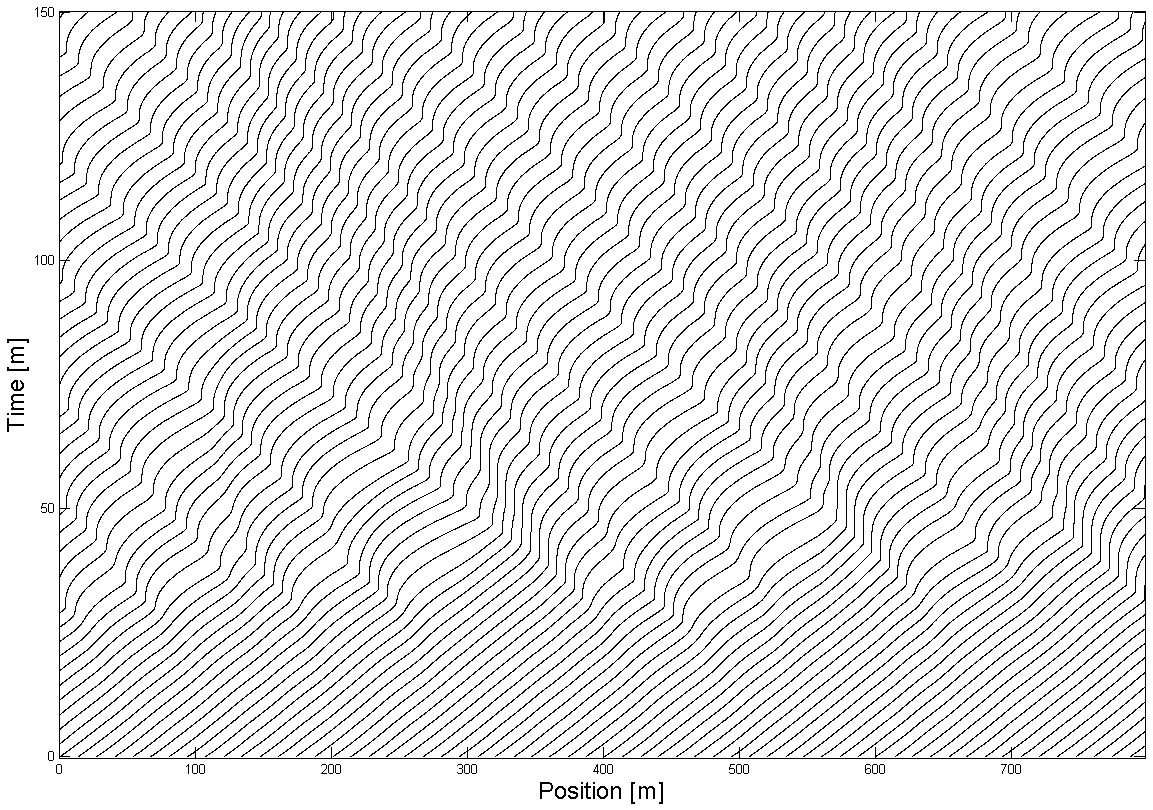
\includegraphics[width=0.8\textwidth]{normal_60cars_50kmh.png}
    \caption{\label{normal_postime}
Absolute position of 60 cars for $ 150 \unit{s} $. Data from simulator. After $ 30 \unit{s} $ phantom jams are emerging.}
    \end{center}
\end{figure}

% Ska vi ha velocityplotten?

\subsection{Comparison of Performance}
We measure performance of the different systems as average traffic flow
$ [\unit{vehicles/h}] $ as a function of average traffic density
$ [\unit{vehicles/km}] $. The speed limit was fixed to $ 50 \unit{km/h} $ in all
experiments. Data is presented in fig \ref{performace}.\\\\

Initially, the performance of all three systems grow linearly as traffic is
light enough to allow all cars to keep maximum allowed speed. As traffic grows
denser, the cars have to slow down to keep constant time headway. All three
system follow the same performance curve until a density of $ 50.0
\unit{vehicles/km} $ is reached. At this point, phantom jams appear in the
\emph{normal driver} system and traffic flow drops dramatically. For the
\emph{Adaptive Cruise Control} system and the \emph{Enhanced Adaptive Cruise
Control} system, phantom jams were first observed at $ 56.3 \unit{vehicles/km} $
and $ 68.8 \unit{vehicles/km} $ respectively. Fig \ref{performance} also shows
that the performance of these two systems is not reduced by the phantom jams
as severely as for the \emph{normal driver}.

\begin{figure}[h!]
    \begin{center}
    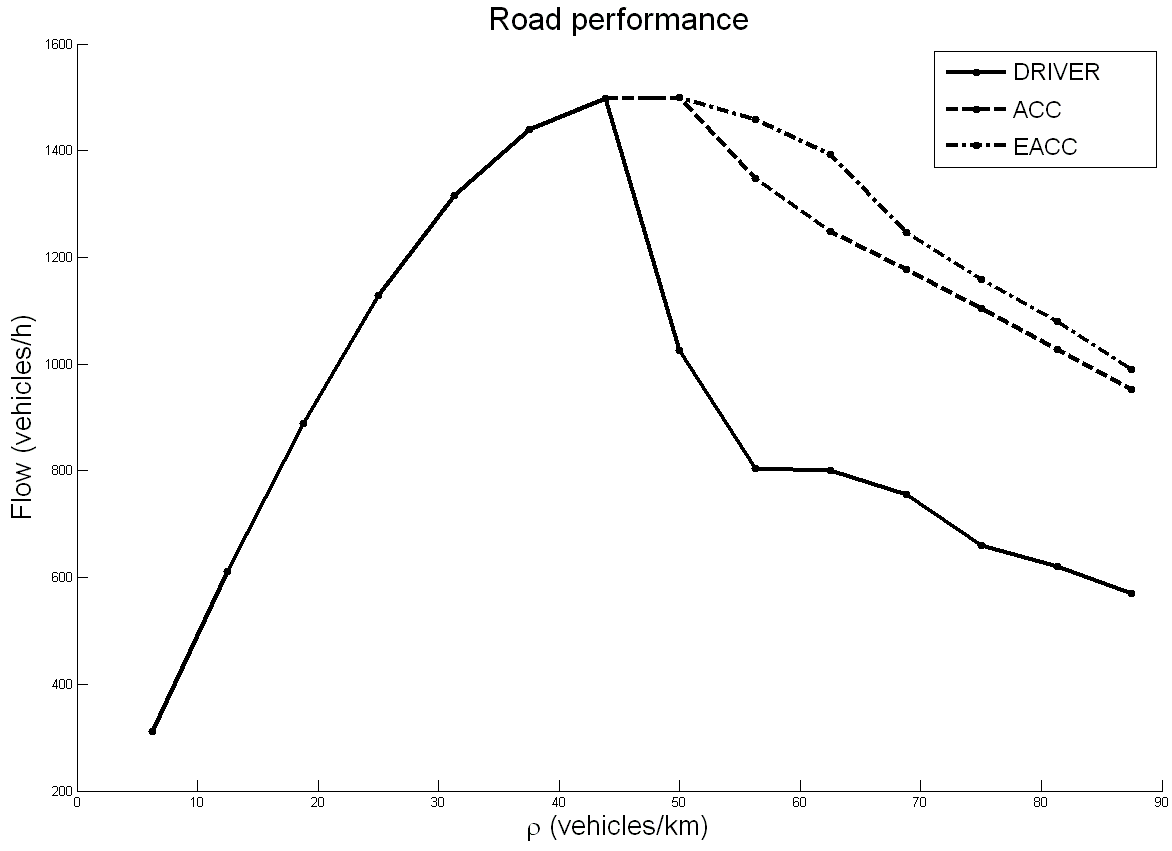
\includegraphics[width=0.8\textwidth]{flowdensity_2.png}
    \caption{\label{performance}
Traffic flow as a function of traffic density. Data from simulator.
$ RoadLength=800 \unit{m} $, $ SpeedLimit=50 \unit{km/h} $, $ TimeHeadway=1.5
\unit{s} $. Traffic flow was measured when traffic conditions had stabilized.}
    \end{center}
\end{figure}




%Discussion
\section{Conclusion}
Real-world traffic systems are complex, composed of light and heavy vehicles,
complex road systems, individual drivers etc. We have chosen to work
with a minimalistic model, still capable of reproducing phantom jams as
observed in real-world traffic.\\\\

We have investigated two systems that show promising results in our
simulations compared to a \emph{normal driver}. The normal driver used in our
simulations is, however, not a normal driver. It is capable of perfectly assessing
the distance to and the velocity of, the vehicle if front of it. All cars also
share the same driver model. In fact, the only thing separating the normal
driver system from the ACC system is the reaction time. We have done some
simulations with mixtures of vehicles with different dynamics and with
non-deterministic driver models. Our impression is that this worsens the
problem with phantom jams, and reduces traffic flow further. We also believe
that ACC and EACC has the ability to stabilize these systems, which more closely
resembles reality, and expect the performance gap to normal drivers to be even
larger in reality. But, more investigations and simulations on the topic is
need.\\\\

So, what's the catch? Using systems such as ACC and EACC in real world
situations to improve road capacity might not be a straight-forward task. G.
Marsden et al. address some of the problems with ACC in \emph{Towards an
understanding of adaptive cruise control} \cite{accCritics}; A lane with ACC
vehicles can experience increased instability, compared with manual driving,
in some traffic situations. For instance, when a manually controlled vehicle
cut in between two ACC vehicles, a sharp deceleration caused by the suddenly
decreased time-gap might start a travelling traffic jam. Also, speed and
traffic capacity has been shown to vary with ACC target time-gaps and
penetration rates.\\\\

% F�rare st�nger idag av systemen i dense traffic - inte avsedda f�r detta
% idag? cite??

%dynamics vary with time-gap and implementeringsgrad % Nu ett stycke med
%nackdelar, sv�righeter och % fr�ga kring effekter av implementeringsgrad:
%Inte helt simpelt - adc kan �ka problem \cite!  Utformning av eadc, f�rslag
%och potential. V�r ide - men finns f�rslag \cite!  eacc beh�ver v�ldigt h�g
%implementeringsgrad eftersom de inte kan kommunicera annars Unders�k effekter
%av implementeringsgrad.

%% Sum -up conclusion
To sum up; Traffic jams constitute a severe problem in the world today.
Building new roads or modifying old road systems to reduce jams and improve
road performance costs huge amounts of money. Our simulations clearly
indicates that automatic or semi-automatic vehicle control systems have the
potential to shift the critical level of traffic density at which phantom jams
occur upwards. Also, the performance penalty for any occurring jams is
reduced. This means that, if such is systems are successfully implemented,
existing roads could handle heavier or much heavier traffic.

\section{Acknowledgements*}
This work was performed as part of the course \emph{Simulation of Complex
Systems} at Chalmers University of Technology. Thanks to our advisor
Kolbj{\o}rn Tunstr{\o}m.



\bibliographystyle{plain}
\bibliography{referenser}
%% APPENDIX
\appendix
\section{GUI}
\label{gui}

\begin{figure}[H]
    \begin{center}
    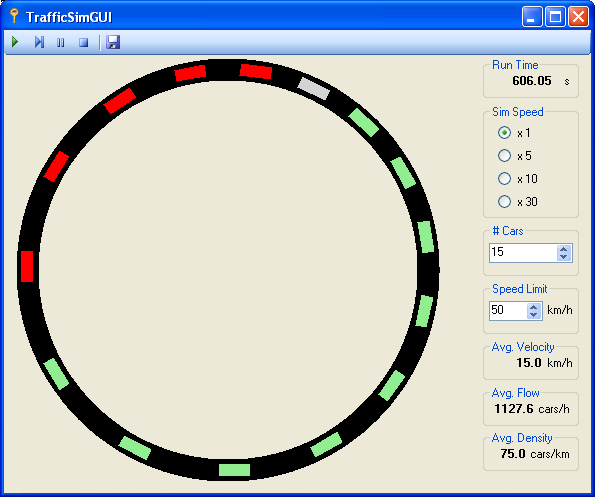
\includegraphics[width=1\textwidth]{simulator2.png}
    \caption{Graphical interface of the simulator which is programmed in C\#. In this figure the road is 200m long with 15 cars. Red cars are braking, green cars are accelerating and the grey car is keeping a constant speed.}
    \end{center}
\end{figure}

\section{Results}
\label{app_postime_plot}
\begin{figure}[H]
    \begin{center}
    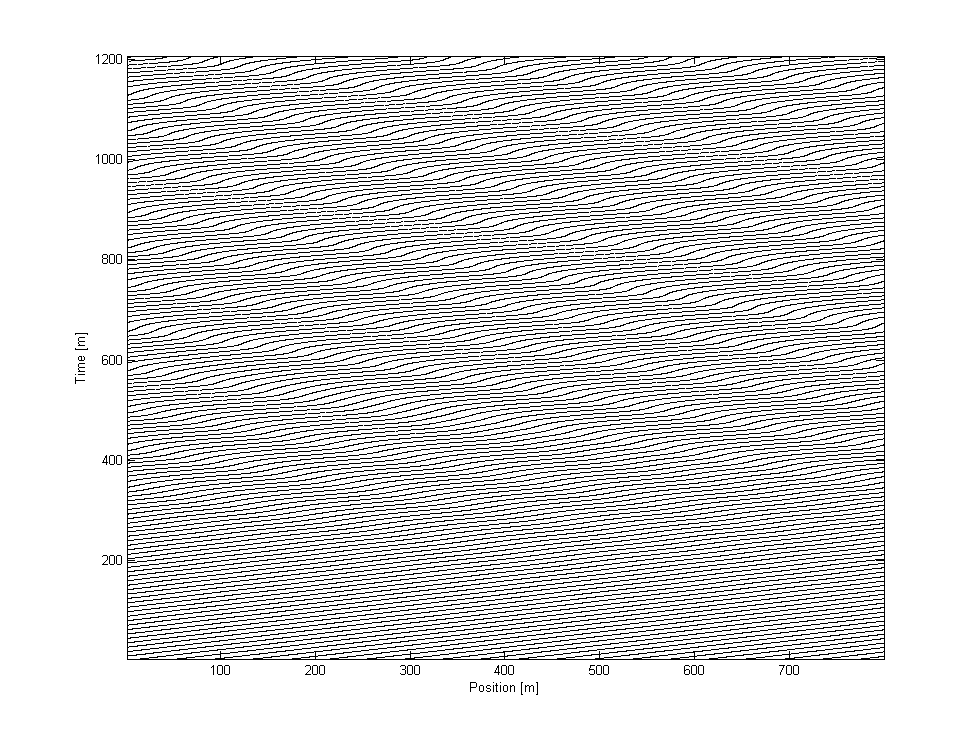
\includegraphics[width=1\textwidth]{acc_60cars_50kmh.png}
    \caption{\label{acc_postime}
Absolute position of 60 cars equipped with adaptive cruise control during $ 1200 \unit{s} $. Data from simulator. After $ 400 \unit{s} $ phantom jams are emerging.}
    \end{center}
\end{figure}

\begin{figure}[H]
    \begin{center}
    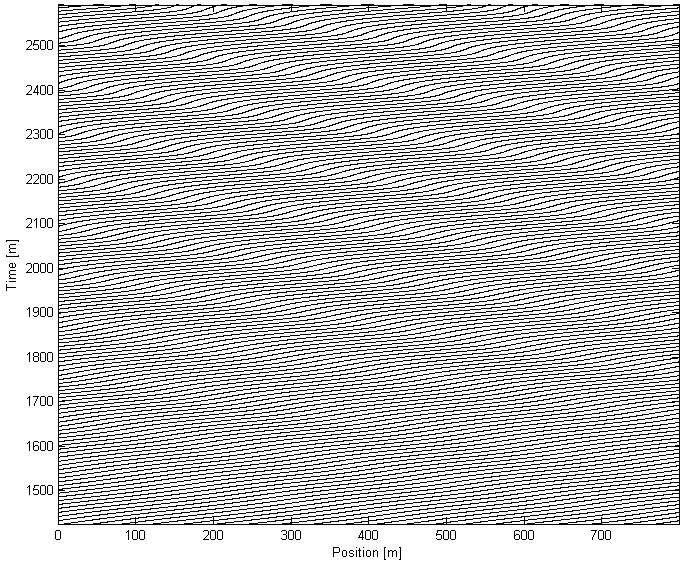
\includegraphics[width=1\textwidth]{eacc_60cars_50kmh.png}
    \caption{\label{eacc_postime}
Absolute position of 60 cars equipped with enhanced adaptive cruise control in the timegep $ 1200 - 2600 \unit{s} $. Data from simulator. After $ 1300 \unit{s} $ phantom jams are emerging.}
    \end{center}
\end{figure}
%%%%%%%%%%%%%%%%%%%%%%%%%%%%%%%%%%%%%%%%%%%%%%%%%%%%%%%%%%%%%%%%%%%%%%%
\end{document}
